%ID: 612068
\begin{blocksection}
\question For the graph below, write the order in which vertices are visited
using the specified algorithm starting from $A$. Break ties by alphabetical
order.  Notice that we have now introduced edge weights to the graph.

\begin{center}
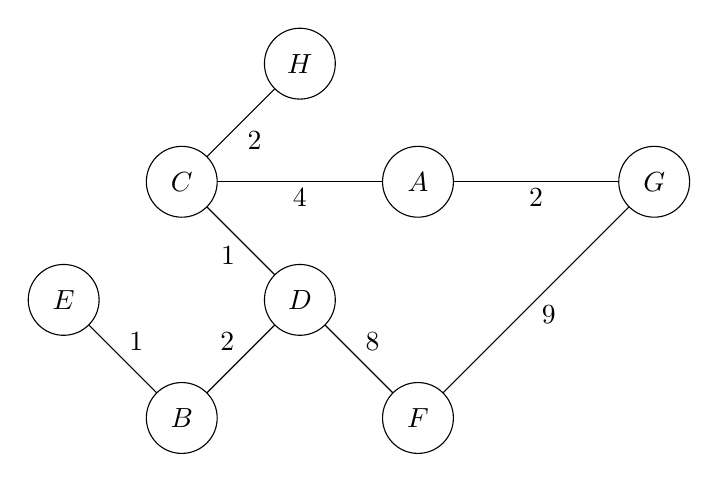
\begin{tikzpicture}[scale=0.15]
\tikzstyle{every node}+=[inner sep=0pt]
\draw [black] (20,-20) circle (3);
\draw (20,-20) node {$C$};
\draw [black] (60,-20) circle (3);
\draw (60,-20) node {$G$};
\draw [black] (40,-40) circle (3);
\draw (40,-40) node {$F$};
\draw [black] (30,-30) circle (3);
\draw (30,-30) node {$D$};
\draw [black] (20,-40) circle (3);
\draw (20,-40) node {$B$};
\draw [black] (10,-30) circle (3);
\draw (10,-30) node {$E$};
\draw [black] (30,-10) circle (3);
\draw (30,-10) node {$H$};
\draw [black] (40,-20) circle (3);
\draw (40,-20) node {$A$};
\draw [black] (42.12,-37.88) -- (57.88,-22.12);
\draw (51.08,-30.48) node [below] {$9$};
\draw [black] (22.12,-22.12) -- (27.88,-27.88);
\draw (23.92,-25.48) node [below] {$1$};
\draw [black] (22.12,-17.88) -- (27.88,-12.12);
\draw (25.52,-16.48) node [right] {$2$};
\draw [black] (23,-20) -- (37,-20);
\draw (30,-20.5) node [below] {$4$};
\draw [black] (43,-20) -- (57,-20);
\draw (50,-20.5) node [below] {$2$};
\draw [black] (37.88,-37.88) -- (32.12,-32.12);
\draw (35.52,-33.52) node [right] {$8$};
\draw [black] (27.88,-32.12) -- (22.12,-37.88);
\draw (24.48,-33.52) node [left] {$2$};
\draw [black] (17.88,-37.88) -- (12.12,-32.12);
\draw (15.52,-33.52) node [right] {$1$};
\end{tikzpicture}
\end{center}

\begin{parts}
\part Pre-Order Depth First Traversal (DFS)
\begin{solution}[0.5in]
Pre-order just means 'first visited', but it's important to make this distinction that 'first visited' means we are looking at the pre-order. 
$A - C - D - B - E - F - G - H$
\end{solution}

\part Breadth First Traversal (BFS)
\begin{solution}[0.5in]
$A - C - G - D - H - F - B - E$
\end{solution}

\part Dijkstra's
\begin{solution}[0.5in]
$A - G - C - D - H - B - E - F$
\end{solution}
\end{parts}
\end{blocksection}
